\section{Screenshots}

\begin{figure}[htb]
    \centering
    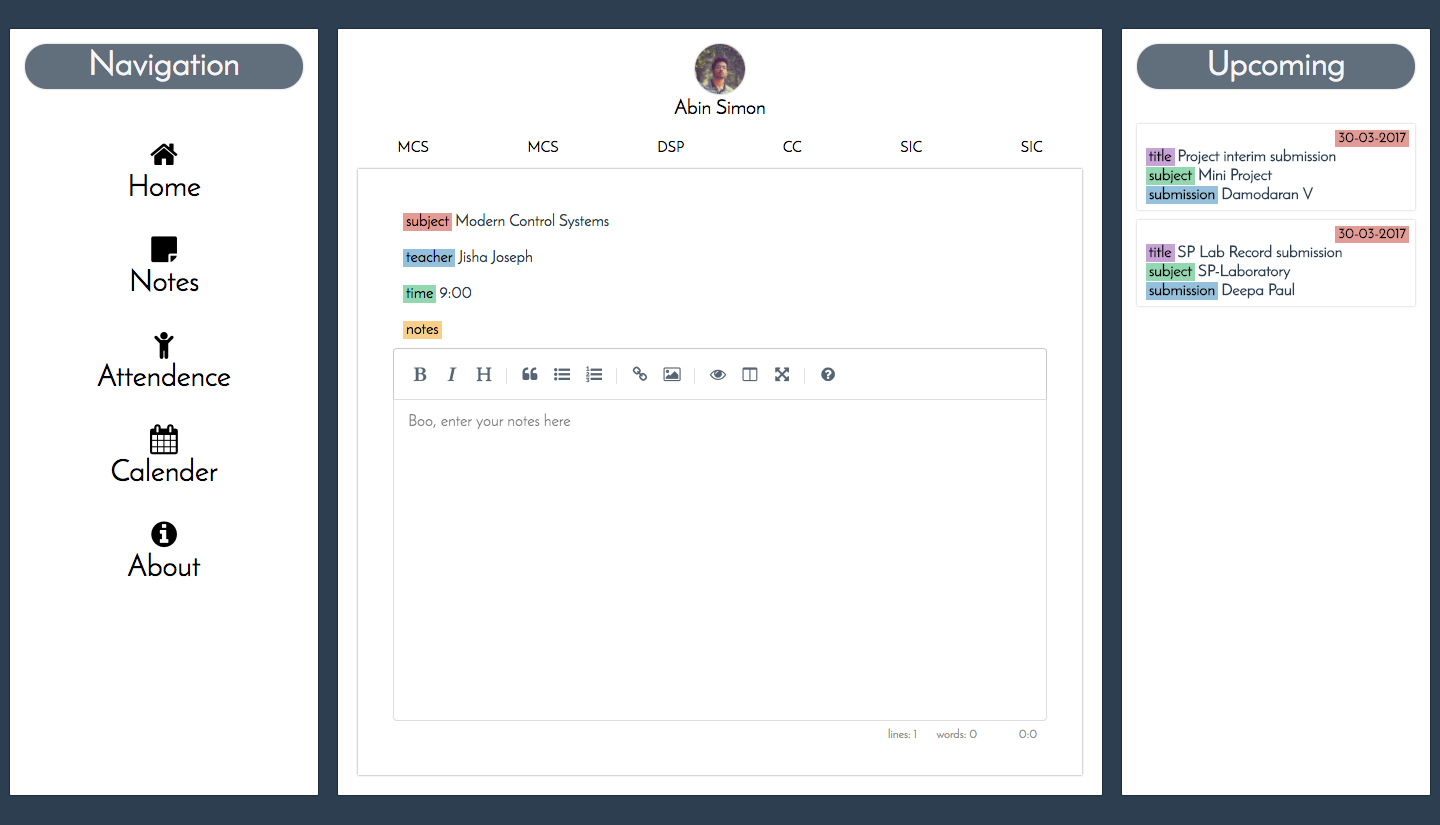
\includegraphics[width=\linewidth]{landingpage.png}
    \caption{Landing page}
    \label{fig:landingpage} % insert suitable label, this is used to refer to a fig from within the text as shown above
\end{figure}

\begin{figure}[htb]
    \centering
    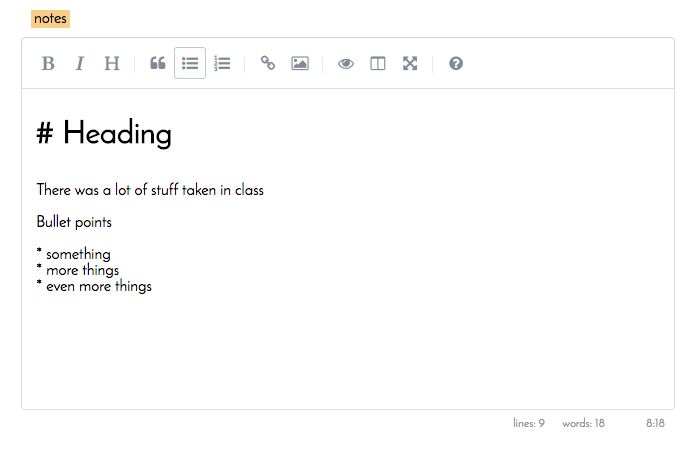
\includegraphics[width=\linewidth]{notesmd.png}
    \caption{Write notes in markdown}
    \label{fig:notesmd} % insert suitable label, this is used to refer to a fig from within the text as shown above
\end{figure}

\begin{figure}[htb]
    \centering
    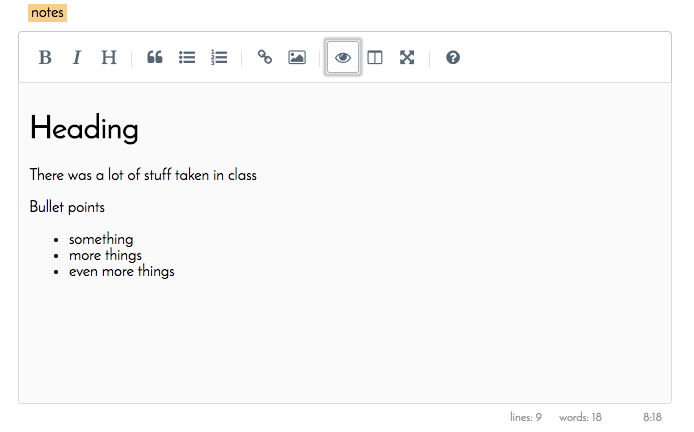
\includegraphics[width=\linewidth]{notescompiled.png}
    \caption{Compiled the written notes to actual contet in place}
    \label{fig:notescompiled} % insert suitable label, this is used to refer to a fig from within the text as shown above
\end{figure}

\begin{figure}[htb]
    \centering
    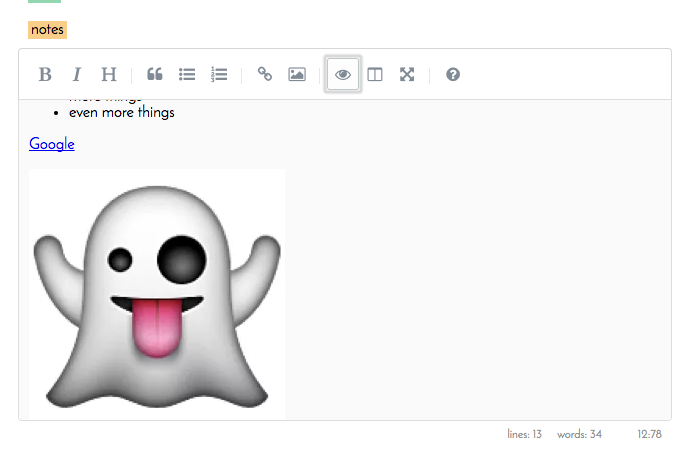
\includegraphics[width=\linewidth]{noteswithimages.png}
    \caption{You can even have notes with images and links}
    \label{fig:noteswithimages} % insert suitable label, this is used to refer to a fig from within the text as shown above
\end{figure}

\begin{figure}[htb]
    \centering
    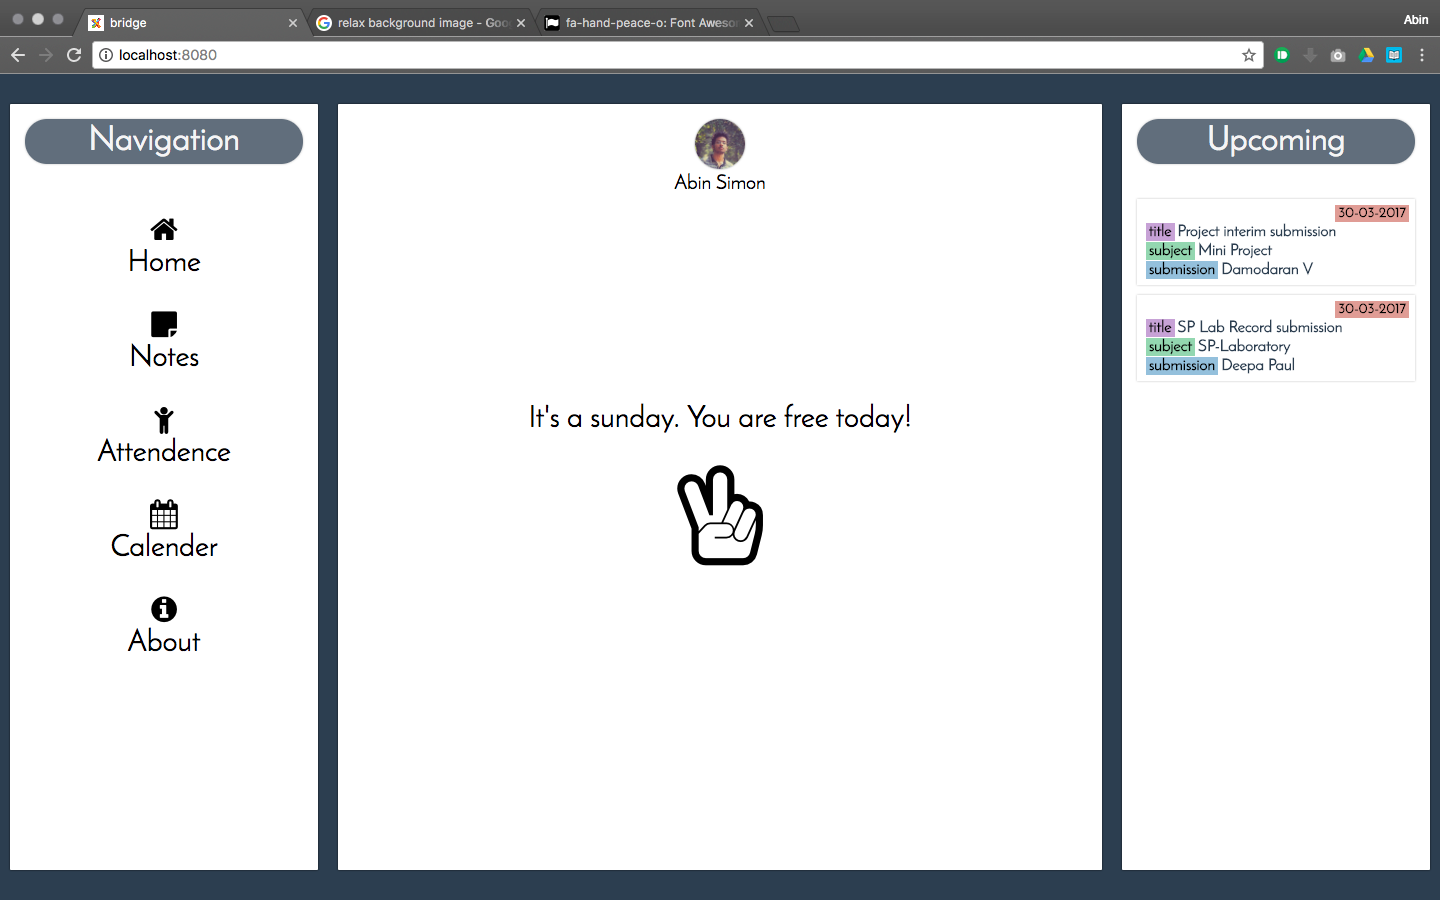
\includegraphics[width=\linewidth]{holiday.png}
    \caption{Landing page on a holiday}
    \label{fig:holiday} % insert suitable label, this is used to refer to a fig from within the text as shown above
\end{figure}

\begin{figure}[htb]
    \centering
    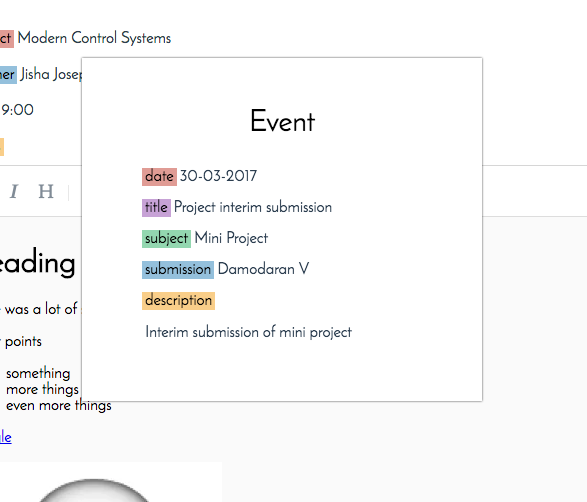
\includegraphics[width=\linewidth]{eventinfo.png}
    \caption{Detailed information about upcoming events}
    \label{fig:eventinfo} % insert suitable label, this is used to refer to a fig from within the text as shown above
\end{figure}

\begin{figure}[htb]
    \centering
    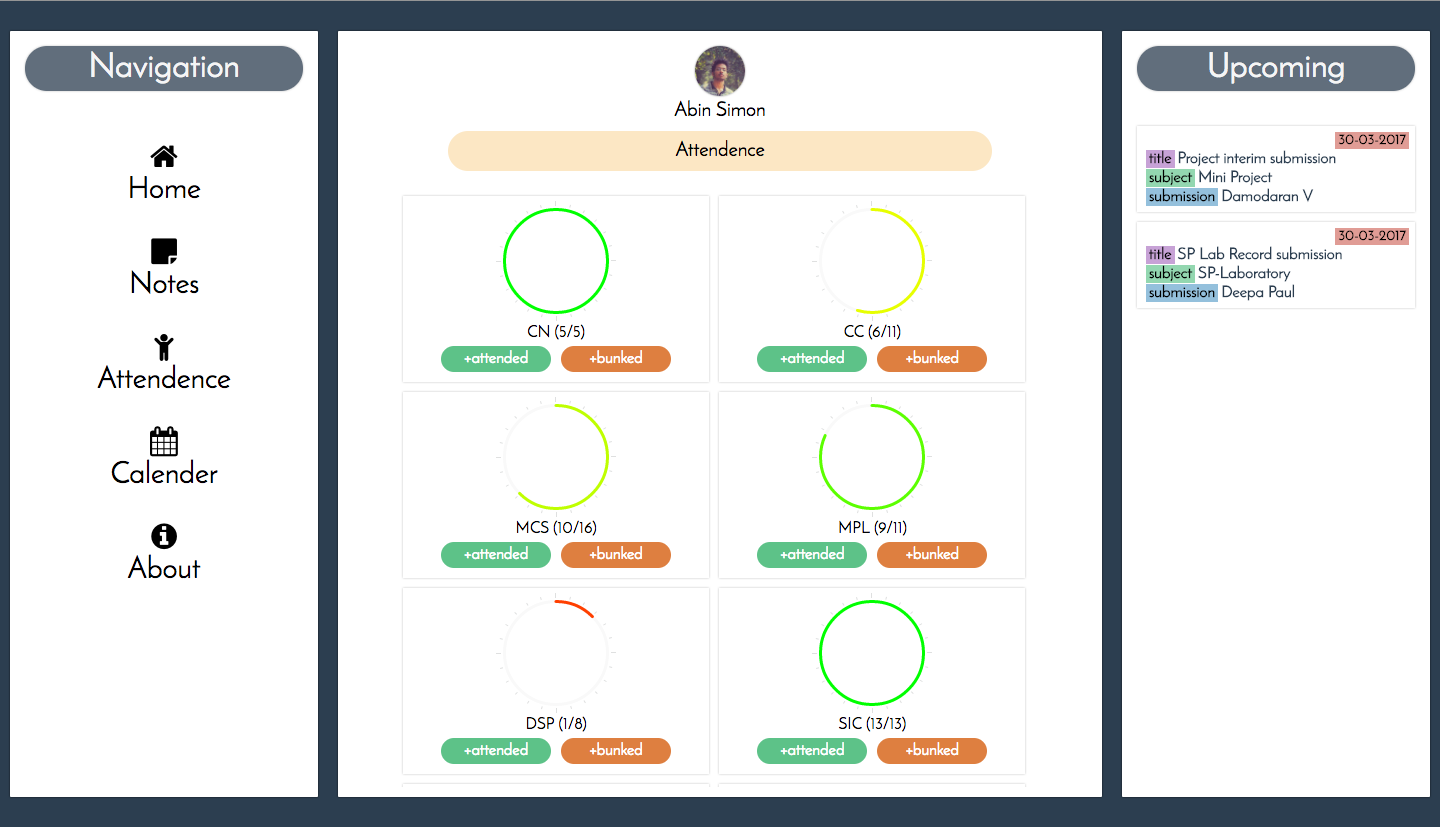
\includegraphics[width=\linewidth]{attendance.png}
    \caption{View and update attendace}
    \label{fig:attendance} % insert suitable label, this is used to refer to a fig from within the text as shown above
\end{figure}

\begin{figure}[htb]
    \centering
    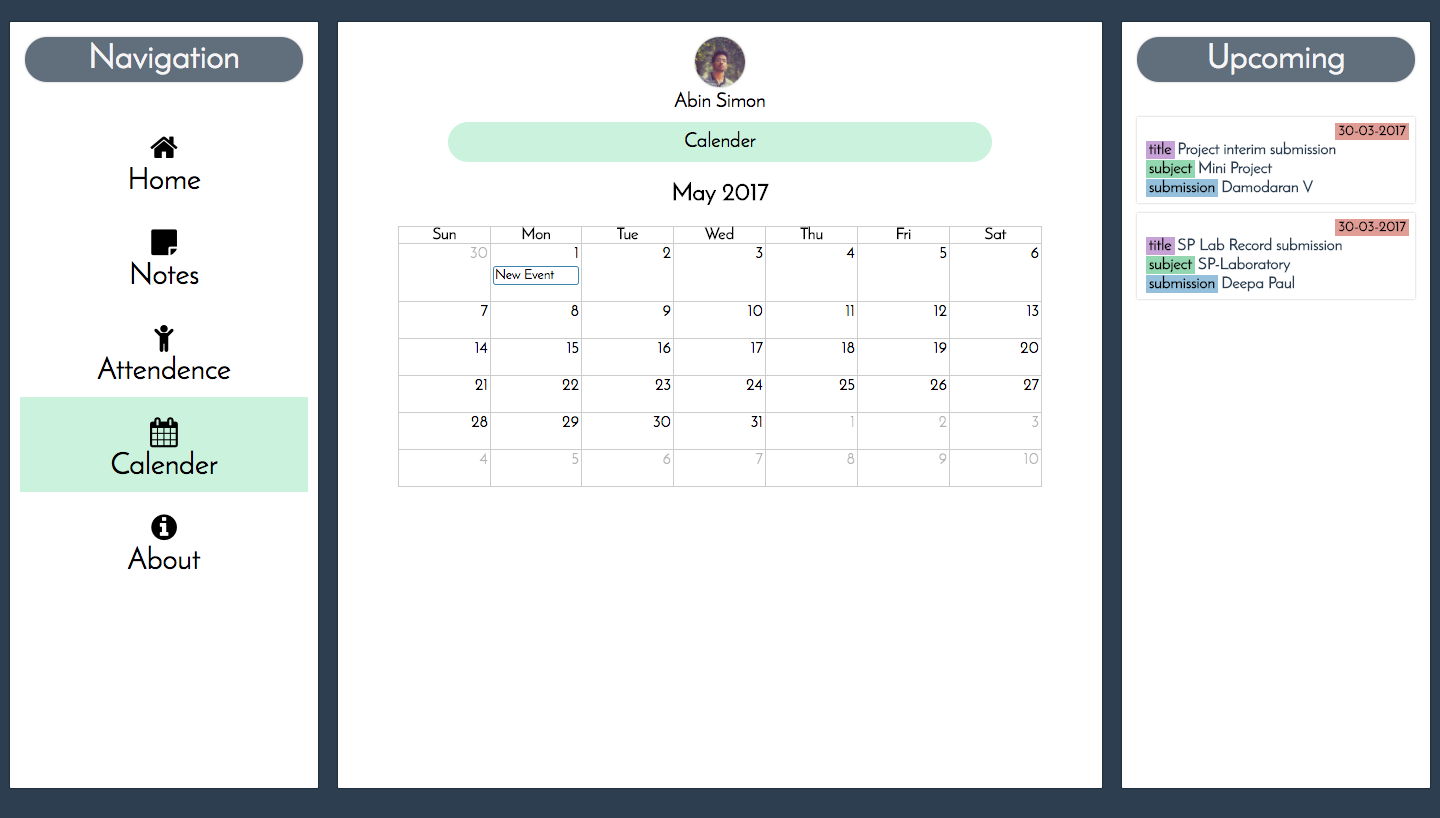
\includegraphics[width=\linewidth]{calendar.png}
    \caption{Calendar entries for events}
    \label{fig:calendar} % insert suitable label, this is used to refer to a fig from within the text as shown above
\end{figure}

\begin{figure}[htb]
    \centering
    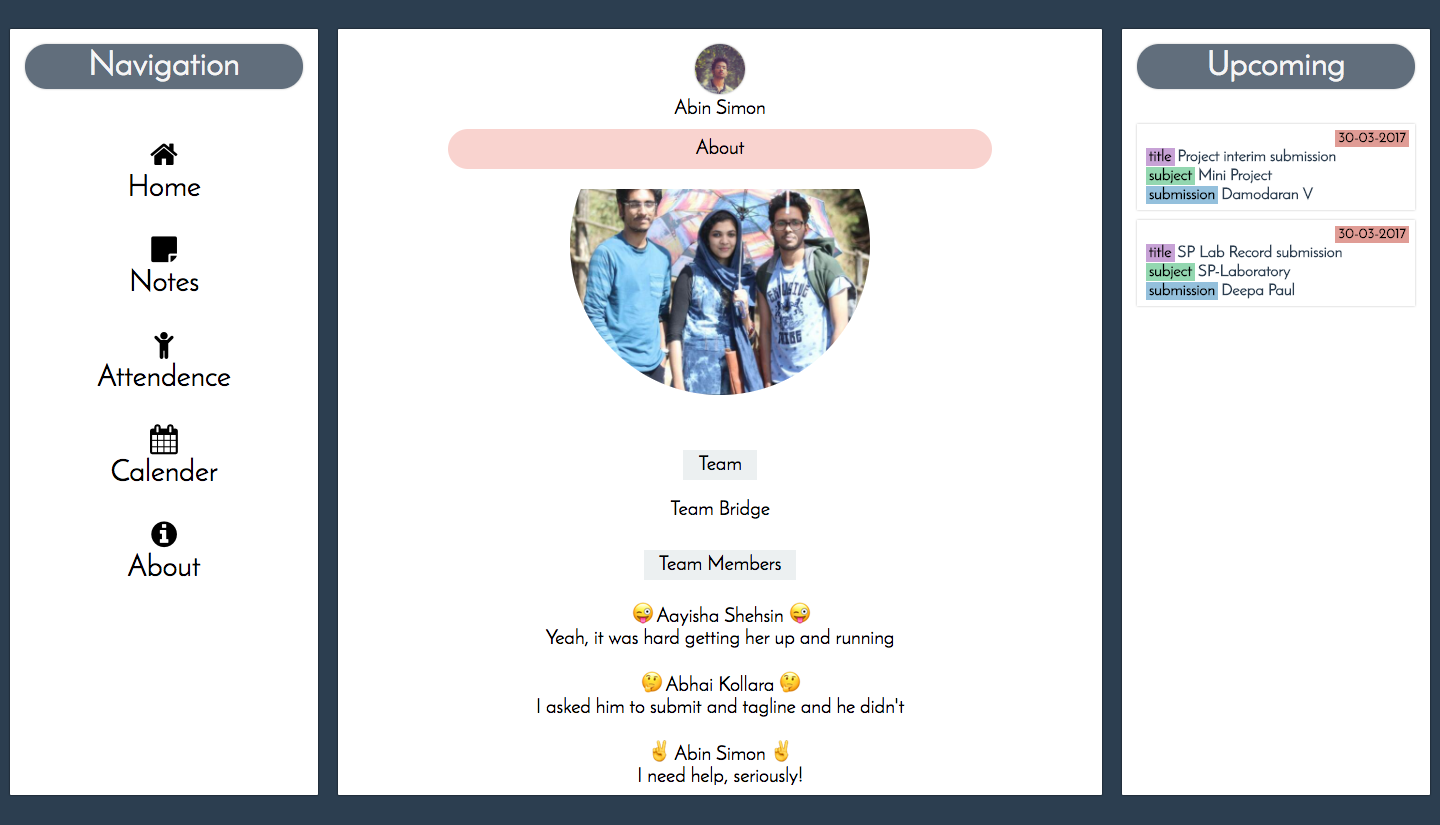
\includegraphics[width=\linewidth]{aboutpage.png}
    \caption{About page}
    \label{fig:aboutpage} % insert suitable label, this is used to refer to a fig from within the text as shown above
\end{figure}

\begin{figure}[htb]
    \centering
    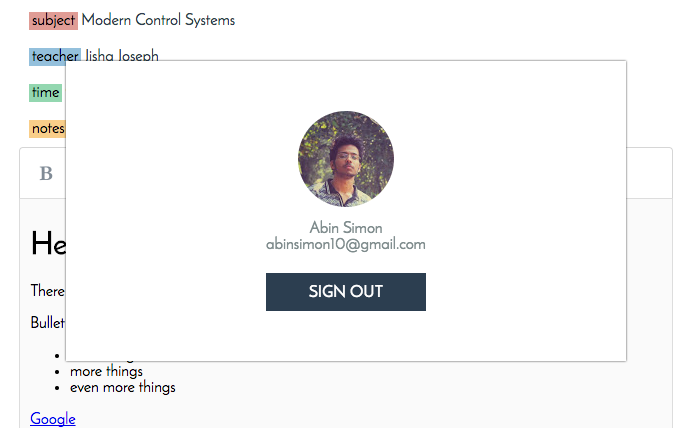
\includegraphics[width=\linewidth]{signoutpopup.png}
    \caption{Popup to sign out of the system}
    \label{fig:signoutpopup} % insert suitable label, this is used to refer to a fig from within the text as shown above
\end{figure}

\begin{figure}[htb]
    \centering
    
\includegraphics[width=\linewidth]{loginpopup.png}
    \caption{Interface for loggin into the app}
    \label{fig:loginpopup} % insert suitable label, this is used to refer to a fig from within the text as shown above
\end{figure}

\begin{figure}[htb]
    \centering
    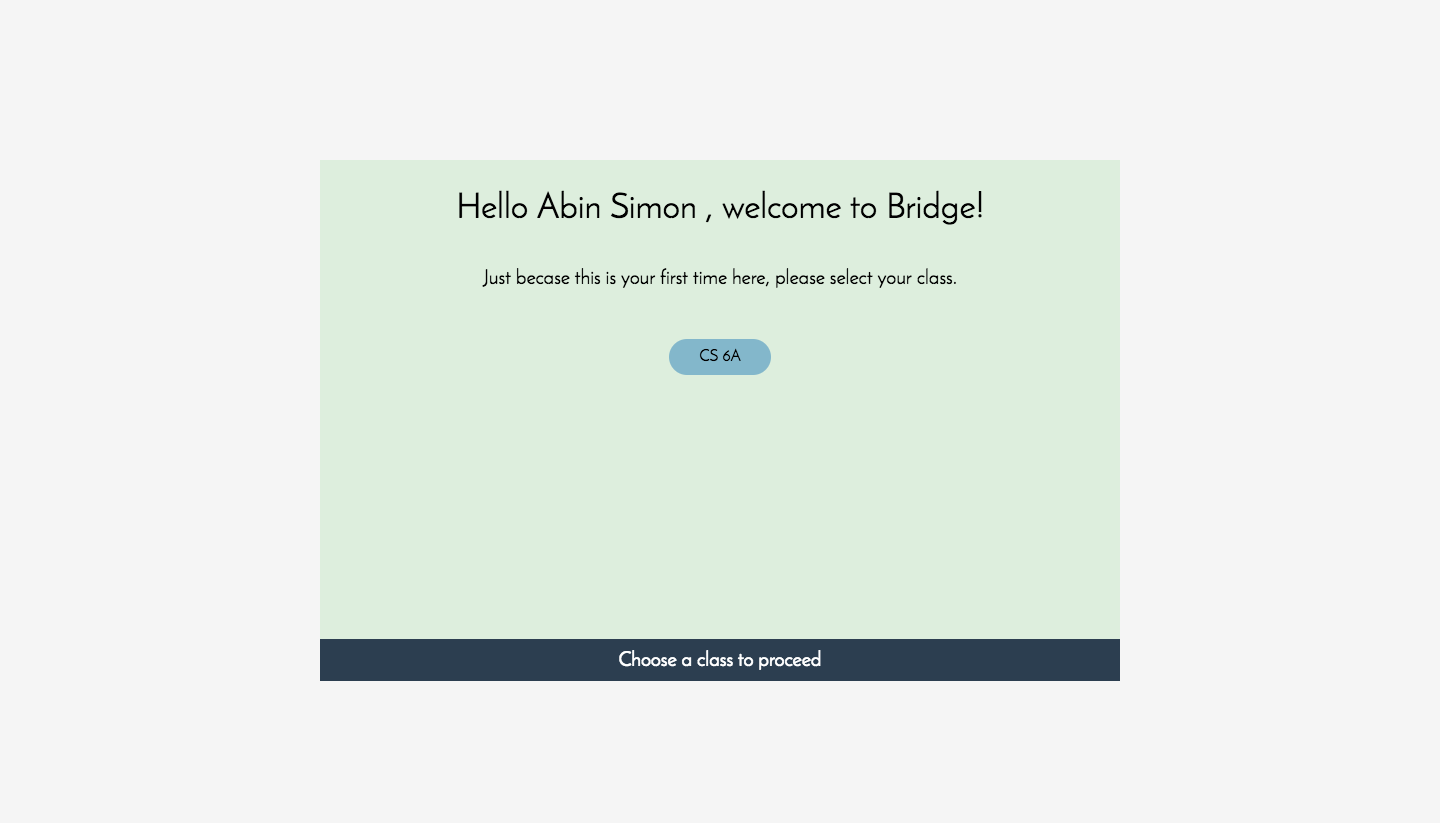
\includegraphics[width=\linewidth]{newuserpopup.png}
    \caption{Interface if the user is a new one so that he can choose a class}
    \label{fig:newuserpopup} % insert suitable label, this is used to refer to a fig from within the text as shown above
\end{figure}

\begin{figure}[htb]
    \centering
    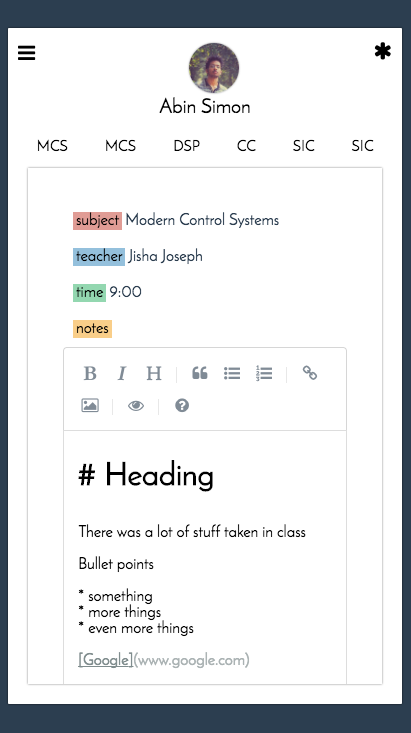
\includegraphics[width=3in]{mobilelanding.png}
    \caption{Landing page on mobile}
    \label{fig:mobilelanding} % insert suitable label, this is used to refer to a fig from within the text as shown above
\end{figure}

\begin{figure}[htb]
    \centering
    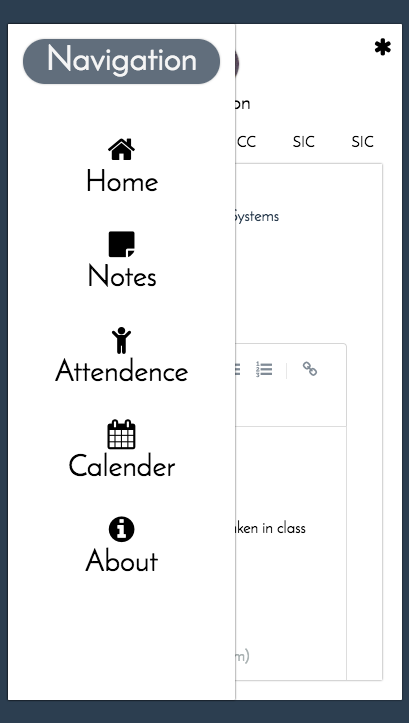
\includegraphics[width=3in]{mobilenav.png}
    \caption{Navigation pane on mobile}
    \label{fig:mobilenav} % insert suitable label, this is used to refer to a fig from within the text as shown above
\end{figure}

\begin{figure}[htb]
    \centering
    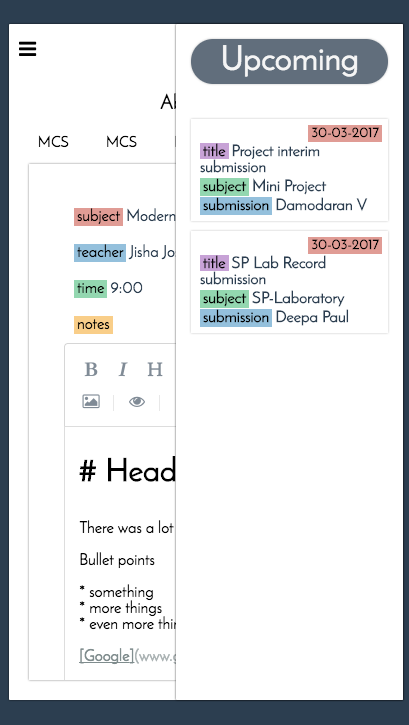
\includegraphics[width=3in]{mobileupcoming.png}
    \caption{Upcoming event display on mobile}
    \label{fig:mobileupcoming} % insert suitable label, this is used to refer to a fig from within the text as shown above
\end{figure}

\begin{figure}[htb]
    \centering
    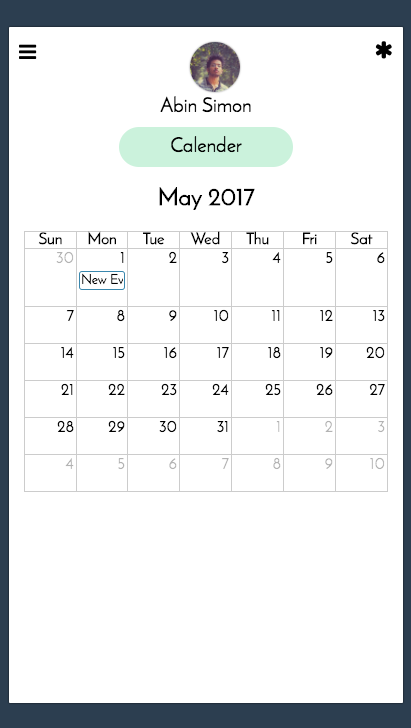
\includegraphics[width=3in]{mobilecalendar.png}
    \caption{Calendar display on mobile}
    \label{fig:mobilecalendar} % insert suitable label, this is used to refer to a fig from within the text as shown above
\end{figure}
